% California Management Review (CMR) Article
% Generative AI and Digital Product Management: Converting Speed into Learning
% Anonymous manuscript submission
% Format: 12-point, double-spaced
% Style: Chicago Manual of Style (18th ed.) Notes format with endnotes
% Word count: ~8,000 words (excluding tables/figures/endnotes)

\documentclass[12pt]{article}

% ============================================
% PACKAGES
% ============================================

\usepackage[utf8]{inputenc}
\usepackage[T1]{fontenc}
\usepackage{lmodern}
\usepackage[english]{babel}
\usepackage{setspace}
\doublespacing

\usepackage{graphicx}
\usepackage[dvipsnames,svgnames,table]{xcolor}

\usepackage{listings}
\lstset{
    basicstyle=\ttfamily\small,
    breaklines=true,
    frame=single,
    backgroundcolor=\color{gray!10},
    xleftmargin=1em,
    framexleftmargin=1em
}

\usepackage{amsmath,amssymb}
\usepackage[colorlinks=false,bookmarks=true,bookmarksnumbered=true]{hyperref}
\usepackage{booktabs,longtable,tabularx,array}
\usepackage{enumitem}
\usepackage{endnotes}
\usepackage{tikz}
\usetikzlibrary{shapes.geometric,arrows.meta,positioning,calc,decorations.pathreplacing}
\let\footnote=\endnote

\usepackage[left=1in, right=1in, top=1in, bottom=1in]{geometry}

% ============================================
% HEADING STYLES
% ============================================

\renewcommand{\section}[1]{%
    \vspace{12pt}%
    \noindent\centerline{\textbf{\uppercase{#1}}}%
    \vspace{6pt}%
}

\renewcommand{\subsection}[1]{%
    \vspace{10pt}%
    \noindent\textbf{#1}%
    \vspace{4pt}%
}

\renewcommand{\subsubsection}[1]{%
    \vspace{6pt}%
    \noindent\textit{\textbf{#1}.} %
}

% ============================================
% DOCUMENT
% ============================================

\begin{document}

\begin{center}
\textbf{\Large The Learning Velocity Advantage: \\ How Generative AI Creates Competitive Advantage Through Faster Learning, Not Better Thinking}
\end{center}

\vspace{12pt}

\section*{Abstract}

Generative AI is reshaping product development, yet productivity gains often fail to improve market outcomes. This article argues that AI's strategic value is not automation or intelligence augmentation but a fundamental reduction in the cost of organizational learning---the \textit{Learning Velocity Advantage}. AI does not improve decisions; it improves the economics of learning under uncertainty. We present a four-stage framework explaining how cost reduction converts to competitive advantage through experimentation expansion, learning acceleration, and compounding. Organizations investing in learning infrastructure---measurement systems, interpretation discipline, decision governance---will convert AI-enabled speed into sustained advantage. Those treating AI as productivity automation will produce mediocrity faster.

\vspace{6pt}

\noindent\textbf{Keywords:} generative AI, learning velocity advantage, experimentation economics, organizational learning, competitive advantage, digital product management

\newpage

% ============================================
% MAIN CONTENT
% ============================================

\section{The Productivity Paradox Executives Cannot Ignore}

Here is a paradox that should unsettle every executive investing in generative AI: teams are shipping faster than ever, yet products are not getting better.

Generative AI tools have arrived with remarkable promise. Teams now draft requirements in minutes instead of weeks. Designers generate dozens of interface variants in hours. Product managers synthesize market research that once required external consultants. Features ship faster. Roadmaps evolve more frequently. Activity increases. But outcomes? Outcomes remain stubbornly unchanged.

A puzzling pattern has emerged across industries: organizations adopting AI become faster at producing product artifacts without becoming better at deciding which artifacts matter.\endnote{Ångström, Rebecka C., Michael Björn, Linus Dahlander, Magnus Mähring, and Martin W. Wallin. ``Getting AI Implementation Right: Insights from a Global Survey.'' \textit{California Management Review} 66, no. 1 (2023): 5--22.} Features ship more quickly, but adoption remains uncertain. Prototypes multiply, but signal from noise does not. Roadmaps change frequently, but strategic clarity declines.

This disconnect reflects a fundamental misunderstanding---one that shapes how most organizations approach AI adoption. The dominant narrative frames AI as a tool for \textit{better thinking}: smarter recommendations, automated analysis, augmented judgment. This narrative is seductive. It is also wrong.

The thesis of this article is different, and its implications are consequential:

\textbf{AI does not create competitive advantage by improving decisions. It creates advantage by lowering the cost of learning under uncertainty.}

This distinction matters because it changes everything about how organizations should adopt AI. Speed without learning is efficient mediocrity. But speed \textit{in service of} learning---running more experiments, failing faster, and compounding insight over time---is how lasting competitive advantage is built. We call this the \textit{Learning Velocity Advantage}.

\section{Two Theories of AI Value---Only One Is Right}

Most organizations adopt AI with an implicit theory: AI will make our people faster, allowing us to do more work with existing resources. Call this the \textit{automation theory}. It is measurable, intuitive, and wrong in a consequential way.

The productivity research on generative AI validates the automation theory's premise while undermining its promise. Studies of GitHub Copilot document significant improvements in task completion speed, particularly for routine, well-defined coding tasks.\endnote{GitHub, ``Research: Quantifying GitHub Copilot's Impact on Developer Productivity and Happiness,'' GitHub Blog, September 2022, https://github.blog/news-insights/research/.} McKinsey research estimates that generative AI could accelerate software product time to market by 20--40 percent.\endnote{McKinsey \& Company, ``Unleashing Developer Productivity with Generative AI,'' June 2023, https://www.mckinsey.com/capabilities/mckinsey-digital/our-insights/unleashing-developer-productivity-with-generative-ai.} IBM documents measurable gains in development cycle compression.\endnote{IBM, ``The CEO's Guide to Generative AI,'' IBM Institute for Business Value, 2023, https://www.ibm.com/thought-leadership/institute-business-value/en-us/report/ceo-generative-ai.} People are, in fact, faster.

Yet these productivity gains do not automatically translate into better products. The Accelerate State of DevOps Report 2024 documents that while AI tools improve deployment frequency and lead time for changes---the velocity metrics---they do not consistently improve change failure rate or mean time to recovery.\endnote{DORA, \textit{Accelerate State of DevOps Report 2024} (Google Cloud, 2024), https://dora.dev/research/.} Speed and quality are not the same. Faster shipping can amplify the impact of poor decisions.

The alternative theory---the \textit{learning theory}---reframes AI's value proposition entirely. Generative AI reduces the cost of producing artifacts: code, designs, requirements, prototypes. But artifacts are not outcomes. Products succeed or fail based on whether they address real user needs and deliver measurable value. That determination requires learning, not just production.

The distinction between experimentation and learning deserves explicit attention: \textit{experimentation is activity; learning is the extraction of actionable insight from that activity}. Organizations can run hundreds of experiments and learn nothing. They can also run a handful of well-designed experiments and fundamentally change their strategic direction. The Learning Velocity Advantage comes not from experiment volume, but from the rate at which experiments produce decisions that compound into market advantage.

\section{Theoretical Foundations}

The Learning Velocity Advantage builds on three foundational streams of organizational research, each of which illuminates a different dimension of how AI transforms competitive dynamics.

\subsection{Exploration and Exploitation}

James March's seminal distinction between exploration (searching for new possibilities) and exploitation (refining existing capabilities) frames a central tension in organizational strategy.\endnote{March, James G. ``Exploration and Exploitation in Organizational Learning.'' \textit{Organization Science} 2, no. 1 (1991): 71--87.} Organizations that over-exploit become competent at obsolete activities; those that over-explore fail to capture returns on their discoveries. The optimal balance depends critically on the cost of exploration---and generative AI fundamentally reduces that cost.

When exploration was expensive, rational organizations favored exploitation. The Learning Velocity Advantage shifts this calculus: cheaper experimentation makes exploration economically viable in contexts where it was previously prohibitive. Organizations can now explore more strategic alternatives before committing to exploitation. The framework thus extends March's insight by identifying a mechanism---AI-enabled cost reduction---that systematically expands the exploration frontier.

\subsection{Dynamic Capabilities}

The dynamic capabilities literature examines how organizations sense opportunities, seize them through resource reconfiguration, and transform existing assets.\endnote{Teece, David J. ``Explicating Dynamic Capabilities: The Nature and Microfoundations of (Sustainable) Enterprise Performance.'' \textit{Strategic Management Journal} 28, no. 13 (2007): 1319--1350.} Sensing---the ability to identify and assess opportunities---has traditionally been constrained by research costs and cognitive limitations. AI accelerates sensing by enabling rapid, low-cost market scanning and hypothesis testing.

More importantly, AI transforms the economics of seizing. Kathleen Eisenhardt's research on strategic decision-making in high-velocity environments showed that faster decisions correlate with better outcomes when organizations use real-time information and multiple simultaneous alternatives.\endnote{Eisenhardt, Kathleen M. ``Making Fast Strategic Decisions in High-Velocity Environments.'' \textit{Academy of Management Journal} 32, no. 3 (1989): 543--576.} The Learning Velocity Advantage operationalizes this insight: AI enables organizations to pursue multiple strategic alternatives simultaneously at lower cost, improving both decision speed and decision quality.

\subsection{Absorptive Capacity}

Cohen and Levinthal's concept of absorptive capacity---the ability to recognize, assimilate, and apply new external knowledge---highlights that learning is not automatic.\endnote{Cohen, Wesley M., and Daniel A. Levinthal. ``Absorptive Capacity: A New Perspective on Learning and Innovation.'' \textit{Administrative Science Quarterly} 35, no. 1 (1990): 128--152.} Organizations require prior related knowledge to benefit from new information. This insight explains why Stage 3 of our framework---Learning Acceleration---is decisive: AI increases the volume of potential learning inputs, but converting inputs to actionable knowledge requires organizational absorptive capacity.

The implication is that AI does not substitute for organizational learning capability; it raises the returns to that capability. Organizations with high absorptive capacity will extract disproportionate value from AI-enabled experimentation. Those with low absorptive capacity will generate data noise, not strategic insight. The Learning Velocity Advantage thus depends on a complementary investment in interpretation infrastructure.

\subsection{Synthesis}

These three streams converge on a coherent implication: AI's strategic value lies in changing the economics of organizational learning, not in replacing human judgment. March's framework explains \textit{why} cheaper exploration matters (it shifts the optimal explore/exploit balance). Dynamic capabilities explain \textit{how} faster learning translates to competitive advantage (through improved sensing and seizing). Absorptive capacity explains \textit{what determines} whether organizations capture value from learning opportunities (prior knowledge and interpretation capability).

The Learning Velocity Advantage framework makes two distinctive contributions to this literature. First, it identifies generative AI as a mechanism that simultaneously affects all three theoretical streams---reducing exploration costs, accelerating sensing and seizing cycles, and increasing the volume of learning opportunities. This cross-cutting impact distinguishes AI from previous technological innovations that typically affected only one dimension.

Second, the framework specifies the organizational infrastructure required to convert AI-enabled speed into learning advantage. While prior research has established the importance of learning capability, the Learning Velocity Advantage framework provides concrete prescriptions: measurement systems that track learning outcomes, decision governance that enables evidence-based pivots, and interpretation capability that extracts signal from noise. These prescriptions transform abstract theoretical concepts into actionable organizational investments.

The following sections develop this framework in detail.

\section{The New Economics of Learning}

Product development has always been constrained by the cost of experimentation. Testing a hypothesis required time: building a prototype, conducting user research, analyzing results. Testing ten hypotheses required ten times the resources. For most organizations, this meant choosing carefully which ideas to test---and those choices were made by executives relying on intuition, politics, or limited data.

Generative AI fundamentally changes this constraint. It does not change \textit{what} organizations can learn; it changes \textit{how much it costs to learn it}. The strategic implications are profound: when learning becomes cheaper, the organizations that learn fastest win.

\subsection{Lower Prototype Cost}

Historically, creating a prototype required specification, design, development, and quality assurance. Bottlenecks were predictable: design hand-offs, code review, bug fixes. With AI assistance, product managers can now generate multiple interface variants in hours. Designers can explore more design spaces. Engineers can produce first-pass implementations faster. The cost per prototype drops by 30--50 percent in many contexts.\endnote{Dell'Acqua, Fabrizio, Edward McFowland III, Ethan R. Mollick, Hila Lifshitz-Assaf, Katherine Kellogg, Saran Rajendran, Lisa Krayer, François Candelon, and Karim R. Lakhani. ``Navigating the Jagged Technological Frontier: Field Experimental Evidence of the Effects of AI on Knowledge Worker Productivity and Quality.'' Harvard Business School Working Paper No. 24-013, September 2023.}

\subsection{Faster Discovery Cycles}

Requirements gathering, market research, and user research are labor-intensive. They are also where speed creates competitive advantage. The first team to understand a market shift or user need often captures disproportionate market share. AI accelerates this cycle. Natural language processing can quickly synthesize customer interviews. Pattern recognition can identify emerging trends in unstructured data. Lead time for market insight shrinks from weeks to days.\endnote{McKinsey \& Company, ``The Economic Potential of Generative AI: The Next Productivity Frontier,'' June 2023, https://www.mckinsey.com/capabilities/mckinsey-digital/our-insights/the-economic-potential-of-generative-ai-the-next-productivity-frontier.}

\subsection{Lower Cost of Failure}

When prototypes were expensive, failure was costly. Failing on a bad idea meant wasted time and resources. This created organizational pressure to de-risk ideas before investing. Teams sought executive approval, conducted extensive upfront analysis, and tried to predict success. With cheaper prototypes, the risk calculus changes. Failing fast becomes rational. Teams can test more ideas and learn from failures cheaply. The organizational learning rate increases.\endnote{Noy, Shakked, and Whitney Zhang. ``Experimental Evidence on the Productivity Effects of Generative Artificial Intelligence.'' \textit{Science} 381, no. 6654 (2023): 187--192.}

Together, these changes reshape the economics of experimentation. The constraint shifts from ``how many ideas can we afford to test?'' to ``how many ideas can we test and still learn from the results?'' This is not a semantic shift. It is a fundamental change in how competitive advantage is created.

\section{The Learning Velocity Framework}

How does AI-enabled speed convert into competitive advantage? Not automatically, and not through productivity alone. We propose a four-stage framework---the Learning Velocity Framework---that explains the mechanism and identifies where most organizations fail. Figure 1 illustrates this progression.

\begin{figure}[htbp]
\centering
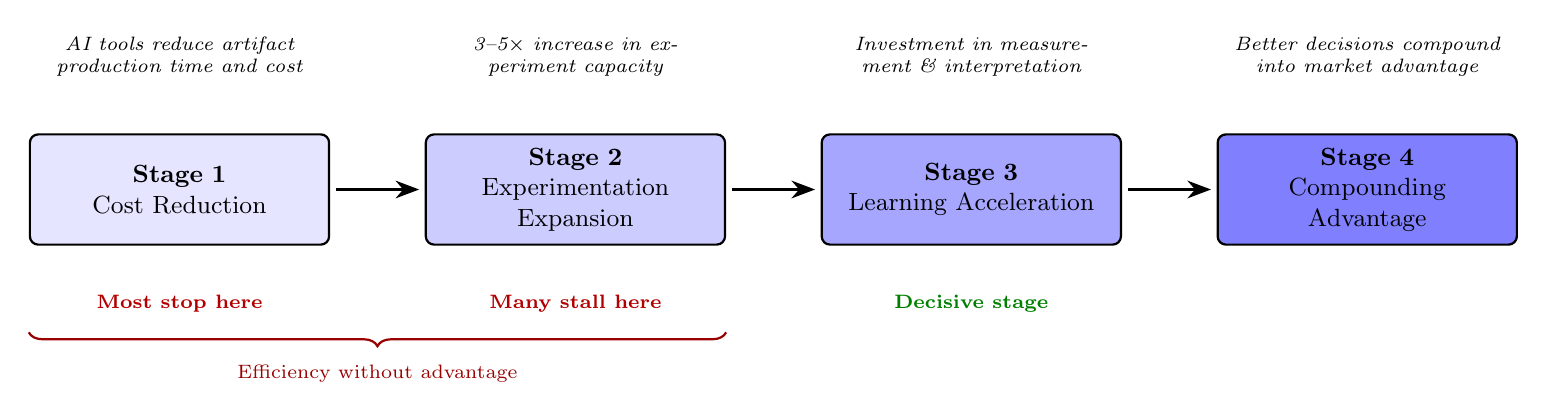
\begin{tikzpicture}[
    stage/.style={
        rectangle,
        rounded corners=3pt,
        draw=black,
        thick,
        minimum width=3.8cm,
        minimum height=1.4cm,
        text centered,
        text width=3.4cm,
        align=center,
        font=\small
    },
    arrow/.style={
        -{Stealth[length=3mm]},
        thick,
        shorten >=2pt,
        shorten <=2pt
    },
    annotation/.style={
        font=\scriptsize\itshape,
        text width=3.5cm,
        align=center
    },
    failpoint/.style={
        font=\scriptsize\bfseries,
        text=red!70!black
    }
]

% Stages
\node[stage, fill=blue!10] (s1) {
    \textbf{Stage 1}\\Cost Reduction
};

\node[stage, fill=blue!20, right=1.2cm of s1] (s2) {
    \textbf{Stage 2}\\Experimentation Expansion
};

\node[stage, fill=blue!35, right=1.2cm of s2] (s3) {
    \textbf{Stage 3}\\Learning Acceleration
};

\node[stage, fill=blue!50, right=1.2cm of s3] (s4) {
    \textbf{Stage 4}\\Compounding Advantage
};

% Arrows
\draw[arrow] (s1) -- (s2);
\draw[arrow] (s2) -- (s3);
\draw[arrow] (s3) -- (s4);

% Annotations above
\node[annotation, above=0.6cm of s1] {AI tools reduce artifact production time and cost};
\node[annotation, above=0.6cm of s2] {3--5$\times$ increase in experiment capacity};
\node[annotation, above=0.6cm of s3] {Investment in measurement \& interpretation};
\node[annotation, above=0.6cm of s4] {Better decisions compound into market advantage};

% Failure points below
\node[failpoint, below=0.5cm of s1] {Most stop here};
\node[failpoint, below=0.5cm of s2] {Many stall here};
\node[failpoint, below=0.5cm of s3, text=green!50!black] {\textbf{Decisive stage}};

% Bracket showing common failure zone
\draw[thick, red!60!black, decorate, decoration={brace, amplitude=5pt, mirror}]
    ([yshift=-1.1cm]s1.south west) -- ([yshift=-1.1cm]s2.south east)
    node[midway, below=8pt, font=\scriptsize, text=red!60!black] {Efficiency without advantage};

\end{tikzpicture}
\caption{The Learning Velocity Framework: Four stages from AI adoption to competitive advantage. Most organizations stop at Stages 1 or 2, capturing productivity gains without sustained competitive differentiation. Stage 3---investment in learning infrastructure---is the decisive transition point.}
\label{fig:framework}
\end{figure}

\subsection{Stage 1: Cost Reduction}

Generative AI reduces the time and cost required to produce product artifacts. This stage is obvious and well-documented. Most organizations recognize this benefit immediately and declare victory. They should not.

\subsection{Stage 2: Experimentation Expansion}

When production costs drop, rational organizations increase the number of experiments. If prototyping cost \$10,000 and took three weeks, teams might conduct four experiments per quarter. If cost drops to \$3,000 and takes one week, teams might conduct twelve. Raw experimentation capacity expands, often by 3--5x.

But here is the trap: \textit{more experiments is not the same as more learning}. Quantity creates the opportunity to learn. Learning itself requires something else entirely---rigorous interpretation, honest analysis, and the organizational discipline to change direction based on evidence. Without these mechanisms, increased experimentation produces noise, not signal.

\subsection{Stage 3: Learning Acceleration---The Decisive Stage}

This stage separates winners from laggards. It is the turning point of the entire argument, and it deserves special emphasis: \textbf{without Stage 3, AI cannot produce sustained competitive advantage}.

Organizations that invest in interpretation infrastructure---measurement systems, analytical capability, and decision governance---amplify the return on increased experimentation. They measure the right metrics. They analyze results rigorously. Most importantly, they change their minds and their roadmaps based on evidence, not on internal consensus or executive intuition.

Organizations that run more experiments without this infrastructure gain nothing but activity. They produce artifacts faster and ship features more frequently, but their cumulative understanding of what customers want does not improve. They accelerate the exploration of wrong paths. Without Stage 3 discipline, increased experimentation amplifies waste, not wisdom.

The distinction is stark: many experiments versus meaningful learning. Only the latter produces advantage.

\subsection{Stage 4: Compounding Advantage}

Organizations that excel at learning under uncertainty make better product decisions. Better decisions compound: better products drive higher retention, lower churn, and stronger network effects. Over time, the learning advantage becomes the market advantage.

This framework explains why some organizations see AI driving dramatic competitive gains while others see efficiency without impact. Most stop at Stage 1 or 2. The leaders reach Stages 3 and 4. The difference is not technology adoption---it is learning infrastructure.

\section{What the Research Shows}

Multiple streams of research converge on a coherent implication that challenges the dominant productivity narrative: generative AI's highest-value application is not strategic reasoning, but enabling rapid, low-cost testing of strategic assumptions.

\subsection{Learning Under Uncertainty}

Organization theory emphasizes that competitive advantage in uncertain environments comes from faster learning, not faster execution.\endnote{Prange, Christiane. ``Agility as the Discovery of Slowness.'' \textit{California Management Review} 63, no. 4 (2021): 27--51.} The 2024 Deloitte State of Generative AI in the Enterprise report confirms that organizations prioritizing learning and capability development from AI adoption see better outcomes than those prioritizing pure automation.\endnote{Deloitte AI Institute, \textit{State of Generative AI in the Enterprise: Now Decides Next} (Deloitte, 2024), https://www2.deloitte.com/us/en/pages/consulting/articles/state-of-generative-ai-in-enterprise.html.}

\subsection{Experimentation as Competitive Strategy}

Research on digital innovation shows that organizations running frequent, low-cost experiments outperform those relying on predictive planning.\endnote{Girod, Stéphane J. G., Julian Birkinshaw, and Christiane Prange. ``Business Agility: Key Themes and Future Directions.'' \textit{California Management Review} 65, no. 4 (2023): 5--21.} The binding constraint is not the ability to run experiments---it is the cost. Generative AI directly addresses this constraint by compressing the time and expense of artifact production.

\subsection{The Productivity Paradox}

The ``productivity paradox'' in technology has long puzzled economists: why do investments in productivity-enhancing technology not always produce proportional improvements in organizational output? Recent research suggests the answer: productivity gains translate into competitive advantage only when organizations restructure workflows and decision-making to leverage the new capability.\endnote{Brynjolfsson, Erik, Danielle Li, and Lindsey R. Raymond. ``Generative AI at Work.'' NBER Working Paper No. 31161, April 2023.} Speed is necessary but insufficient. Organizations must build decision infrastructure to extract learning from speed.

\subsection{Strategic Limitations of Current AI}

Research testing generative AI on strategic tasks found that while AI excels at data synthesis and information retrieval, it remains limited on tasks requiring multi-step reasoning and human behavioral understanding.\endnote{Lechner, Christoph, Nikolaus Lang, Siegfried Handschuh, Olivier Bouffault, and Julian Cooper. ``Can GenAI Do Your Next Strategy Task? Not Yet.'' \textit{California Management Review} 67, no. 1 (2024): 54--77.} This constraint, far from limiting AI's value, clarifies its comparative advantage: AI excels in execution-adjacent work---requirements, prototyping, initial analysis---exactly the work that powers high-velocity experimentation. Strategic reasoning remains a human responsibility.

\subsection{What the Evidence Collectively Implies}

Taken together, these findings point to a single conclusion: AI's strategic value lies not in thinking but in testing. The organizations that will capture disproportionate value from AI are not those with the best AI tools or the fastest deployment. They are the organizations that use AI-enabled speed to run more experiments, extract signal from results with discipline, and change direction based on evidence. The Learning Velocity Advantage is not about artificial intelligence. It is about organizational intelligence---specifically, the capacity to learn faster than competitors under conditions of uncertainty.

\section{The Learning Velocity Advantage in Practice: A Case Illustration}

The following case illustrates how the Learning Velocity Framework operates in practice. Details have been altered to preserve confidentiality, but the organizational dynamics and outcomes reflect documented patterns across multiple AI adoption initiatives.

\subsection{Context: A Mid-Market Financial Services Firm}

A regional financial services company (``Meridian Financial,'' a pseudonym) faced intensifying competition from digital-first entrants. Customer acquisition costs had risen 40 percent over three years while retention rates declined. The executive team authorized a significant investment in generative AI tools, expecting to accelerate product development and reduce operating costs.

\subsection{Stage 1: Rapid Productivity Gains}

Initial results exceeded expectations. Meridian's product teams used AI tools to generate customer journey maps, draft requirements documents, and create interface prototypes. Tasks that previously required two to three weeks compressed to two to three days. The Chief Digital Officer reported a 60 percent reduction in time-to-prototype, and the initiative was celebrated as an early success.

\subsection{Stage 2: Experimentation Expansion---and the First Warning Signs}

Energized by productivity gains, teams increased experimentation. Prototype volume rose from roughly eight per quarter to over thirty. New feature concepts proliferated. Roadmaps expanded. Activity metrics surged.

But six months into the initiative, troubling patterns emerged. Despite tripling experiment volume, customer satisfaction scores remained flat. Feature adoption rates showed no improvement. Several high-profile launches underperformed. Teams were producing more artifacts but not making better product decisions. Meridian had reached Stage 2---and stalled.

\subsection{Stage 3: The Learning Infrastructure Investment}

A cross-functional review surfaced the root cause: Meridian lacked the infrastructure to learn from increased experimentation. Teams generated prototypes rapidly but measured success inconsistently. Customer feedback was collected sporadically. Most critically, no decision governance existed---experiments concluded without clear criteria for what constituted success or failure, and teams defaulted to executive intuition when results were ambiguous.

The Chief Digital Officer made a consequential decision: pause new AI tool adoption and invest in learning infrastructure. Over four months, Meridian implemented three changes:

\textit{Standardized measurement.} Every experiment required predefined success metrics tied to customer outcomes (adoption rate, task completion, retention impact), not activity metrics (features shipped, prototypes created). A central dashboard tracked experiment outcomes, enabling cross-team pattern recognition.

\textit{Decision governance.} The product organization established explicit decision rules: experiments showing statistically significant positive impact on primary metrics would advance; those showing neutral or negative impact would terminate, regardless of executive enthusiasm. Ambiguous results triggered predefined follow-up experiments rather than committee debate.

\textit{Interpretation capability.} Meridian hired two data scientists specifically tasked with experiment analysis---not to build models, but to rigorously interpret results and distinguish signal from noise. Weekly ``learning reviews'' replaced monthly status meetings, with explicit focus on what the organization had learned rather than what it had shipped.

\subsection{Stage 4: Compounding Returns}

The results emerged gradually, then dramatically. Within two quarters of implementing learning infrastructure, Meridian's feature success rate---the percentage of shipped features achieving target adoption---rose from 23 percent to 41 percent. More importantly, teams began killing poor ideas faster. The average time from negative experiment result to roadmap pivot dropped from eleven weeks to three weeks.

Eighteen months after the initial AI investment, Meridian's customer acquisition costs had declined 15 percent while retention rates improved. The competitive gap with digital-first entrants narrowed measurably. The CEO attributed the turnaround not to AI tools but to ``finally learning faster than our competitors.''

\subsection{The Generalizable Lesson}

Meridian's experience illustrates the framework's central claim: AI-enabled productivity gains are necessary but insufficient for competitive advantage. The decisive factor was not the sophistication of AI tools or the speed of artifact production---it was the organizational commitment to convert increased experimentation into systematic learning. Without Stage 3 investment, Meridian would have remained trapped in Stage 2, producing more mediocrity faster. With it, the organization reached Stage 4, where learning compounds into sustained market advantage.

\section{Implications for Leaders}

\subsection{What Leaders Get Wrong}

Before discussing what to do, it is worth naming what not to do. Three errors recur with striking consistency across organizations adopting AI:

\textit{Treating AI as a productivity tool rather than learning infrastructure.} When leaders frame AI adoption as ``doing more with less,'' they optimize for velocity metrics---features shipped, deployment frequency, lines of code. These metrics capture activity, not advantage. The Learning Velocity Advantage requires measuring learning: hypotheses validated, assumptions overturned, time from evidence to decision.

\textit{Investing in experimentation capacity without interpretation capability.} Organizations increase experiment volume by 300 percent while retaining monthly review cadences, consensus-seeking decision processes, and executive intuition as the tie-breaker. Result: data noise, not insight. Experimentation without interpretation is just expensive chaos.

\textit{Assuming that evidence changes decisions automatically.} Even with perfect data showing that a different approach would work, people do not change decisions without explicit authority and incentives. Learning requires changing minds. Changing minds requires organizational permission. Leaders who do not address the politics of evidence-based decision-making will not capture the Learning Velocity Advantage, regardless of their AI investments.

\subsection{Reframe AI Adoption as Learning Infrastructure}

The first actionable implication is conceptual: frame AI adoption not as ``how do we do more with less?'' but as ``how do we learn faster?'' This reframing changes everything.

Instead of asking ``which AI tools will let our team ship 20 percent faster?'', ask ``which AI tools will let us run twice as many experiments and extract signal faster?'' Instead of measuring success by velocity metrics, measure success by learning metrics: hypotheses tested per quarter, time from assumption to decision, feature adoption rate, and actual impact on key business outcomes.

\subsection{Build Measurement Infrastructure First}

Increased experimentation creates value only with strong measurement. Before adopting AI to accelerate prototyping, invest in instrumentation. Define leading and lagging indicators. Establish baselines. Ensure that every experiment produces actionable data.

Many organizations measure vanity metrics (features shipped, users invited to beta) rather than impact metrics (usage, retention, revenue). AI amplifies whatever you measure. Measure the wrong things, and you amplify mediocrity.

\subsection{Create Decision Governance}

More experiments require more decisions---and faster ones. Organizations should establish explicit decision criteria: When do we declare an experiment a success? When do we cut losses and pivot? Who decides? What evidence do we require?

Without explicit decision rules, organizations fall into predictable traps: analysis paralysis (running endless experiments without deciding) or randomness (making decisions inconsistently). AI-enabled experimentation requires both speed and rigor.

\subsection{Additional Pitfalls to Avoid}

Beyond the strategic errors described above, two tactical pitfalls deserve attention:

\textit{Equating experimentation volume with learning.} It is possible to run 50 experiments per quarter while learning nothing. This happens when experiments lack falsifiable hypotheses, results are not systematically documented, or failures trigger blame. Instead, structure experiments around specific learning questions. Require hypotheses before execution. Create psychological safety for honest failure analysis.

\textit{Using AI to optimize existing strategy rather than test new strategies.} Speed amplifies whatever direction you are heading. Organizations implement this mistake by using AI to execute current plans faster, then wonder why they are not becoming more strategic. Instead, deliberately use AI-enabled experimentation to test strategic alternatives---questions like ``If we entered this customer segment, what would we need to build?'' become low-cost hypothesis tests rather than expensive business cases.

\subsection{Protect Experimentation from Politics}

When experiments are expensive, executives often control which ideas get tested. When experiments are cheap, this changes. More experiments should come from frontline teams---designers, engineers, product managers---who see customer problems directly.

However, cheap experimentation creates new risk: the risk of politicization. If a team's pet idea fails, they might blame the experiment design rather than the idea. If a successful experiment threatens an executive's existing roadmap, they might dismiss it as lucky. Protect experimentation from organizational politics by establishing clear norms: all experiments are treated as bets, not truths; outcomes are observed neutrally; surprising results are celebrated as learning opportunities.

\subsection{Invest in Organizational Learning Capability}

The highest-impact organizations will be those that excel at extracting learning from data. This requires statisticians or data scientists who understand experimental design, product managers trained in hypothesis-driven thinking, engineers comfortable with instrumentation and telemetry, and executives who change their minds based on evidence. These capabilities cannot be outsourced. They must be developed internally.

\subsection{Learning Velocity Diagnostic}

To help leaders assess their organization's position and readiness, we offer the following diagnostic questions. Organizations should honestly evaluate each dimension, recognizing that the Learning Velocity Advantage depends on capability across all four areas.

\begin{table}[htbp]
\centering
\small
\caption{Learning Velocity Diagnostic: Seven Questions for Assessing Organizational Readiness}
\label{tab:diagnostic}
\begin{tabularx}{\textwidth}{@{}p{0.5cm}X@{}}
\toprule
\multicolumn{2}{@{}l}{\textbf{Experimentation Capacity}} \\
\midrule
1. & How many product hypotheses did your organization test last quarter? Has this number increased since adopting AI tools? \\
2. & What is the average elapsed time from idea conception to testable prototype? \\
\addlinespace
\multicolumn{2}{@{}l}{\textbf{Measurement Infrastructure}} \\
\midrule
3. & Does every experiment have predefined success criteria established \textit{before} execution begins? \\
4. & Can you distinguish experiments that succeeded from those that failed based on customer outcome data (not stakeholder opinion)? \\
\addlinespace
\multicolumn{2}{@{}l}{\textbf{Decision Governance}} \\
\midrule
5. & When experiment results contradict executive expectations, what happens? Is there an explicit process, or does intuition prevail? \\
6. & What is the average time from conclusive experiment result to roadmap decision? Is this measured? \\
\addlinespace
\multicolumn{2}{@{}l}{\textbf{Learning Culture}} \\
\midrule
7. & In the past quarter, name three significant product decisions that changed based on experimental evidence. If you cannot, why not? \\
\bottomrule
\end{tabularx}
\end{table}

\textbf{Interpreting Results.} Organizations that struggle to answer questions 1--2 are likely stuck at Stage 1 (productivity gains without expanded experimentation). Those answering 1--2 but struggling with 3--4 have reached Stage 2 (experimentation expansion without measurement). Difficulty with 5--6 indicates the Stage 3 bottleneck (measurement without decision governance). Only organizations that can clearly answer all seven questions---including providing concrete examples for question 7---have built the infrastructure for Stage 4 compounding.

The diagnostic is not a scorecard but a conversation starter. Leaders should use these questions to identify specific capability gaps and prioritize infrastructure investments accordingly. The most common pattern is strong performance on questions 1--2 (AI tools deliver productivity gains) combined with weak performance on questions 5--7 (organizational processes have not adapted). This pattern predicts Stage 2 stagnation.

\section{Risks and Boundary Conditions}

This framework comes with important caveats that leaders should consider carefully.

\subsection{Experimentation Exhaustion}

Running constant experiments can exhaust teams and create a culture of endless iteration. Some products require sustained focus on execution, not perpetual experimentation. The framework works best in early-stage products, new features, or uncertain markets. It works less well in mature products where the challenge is polish and reliability rather than learning.

Leaders must recognize that experimentation velocity is not infinitely scalable. Teams have finite cognitive bandwidth for interpreting results and changing direction. Organizations should monitor for signs of experimentation fatigue: declining experiment quality, superficial analysis, or resistance to pivoting despite clear evidence. The Learning Velocity Advantage requires sustainable learning rhythms, not relentless experimentation.

\subsection{Context-Dependent Assumptions}

The framework assumes that product success is uncertain and outcomes can be measured. It works poorly in domains where measurement is difficult (e.g., enterprise software with long sales cycles) or where customer needs are well-known (e.g., regulated financial products). In these contexts, AI's value is more about execution efficiency than learning acceleration.

\subsection{Data Privacy and Governance}

Rapid experimentation generates data. That data must be managed carefully. Organizations must ensure compliance with privacy regulations, proper data governance, and ethical use of customer information. AI amplifies these risks by enabling rapid, at-scale experimentation.\endnote{National Institute of Standards and Technology, \textit{Artificial Intelligence Risk Management Framework (AI RMF 1.0)} (Gaithersburg, MD: NIST, January 2023), https://doi.org/10.6028/NIST.AI.100-1.}

\subsection{Organizational Culture and Change Management}

The Learning Velocity Advantage requires cultural transformation, not merely tool adoption. Organizations with strong hierarchical cultures, where challenging executive judgment carries career risk, will struggle to implement evidence-based decision governance. The framework assumes that organizations can create psychological safety for honest interpretation of experimental results---an assumption that fails in blame-oriented cultures.

Similarly, organizations with entrenched functional silos may find cross-functional learning difficult. When product, engineering, and design teams optimize for their own metrics rather than shared learning outcomes, the interpretation infrastructure fragments. The organizational redesign required to capture the Learning Velocity Advantage may exceed what many organizations can accomplish within typical AI adoption timelines.

\section{Future Research Directions}

The Learning Velocity Advantage framework opens several avenues for future inquiry. First, researchers should examine the relationship between experimentation velocity and organizational learning capacity. At what point does increased experimentation overwhelm interpretation infrastructure? Is there an optimal experimentation rate that varies by industry, organization size, or product maturity?

Second, the framework's boundary conditions deserve empirical investigation. Which industries and contexts benefit most from learning acceleration versus execution efficiency? How do regulatory environments, competitive dynamics, and customer characteristics moderate the framework's applicability?

Third, longitudinal research should examine whether organizations can sustain Stage 4 compounding over extended periods. Do learning advantages erode as competitors adopt similar approaches? What organizational capabilities predict sustained learning velocity rather than temporary advantage?

Finally, researchers should investigate the microfoundations of interpretation capability. What specific skills, processes, and organizational structures enable organizations to extract signal from experimental noise? How do successful organizations balance statistical rigor with decision speed? These questions connect the Learning Velocity Advantage to broader research on organizational learning, dynamic capabilities, and evidence-based management.

\section{Conclusion: The Learning Economics of Competitive Advantage}

Generative AI is reshaping product development. But the arc from AI adoption to competitive advantage is not automatic. It runs through organizational learning.

The competitive winners will not be the organizations that adopt AI first or ship features fastest. They will be the organizations that use AI to \textit{learn} faster---running more experiments, extracting signal from noise with rigor, making decisions decisively, and compounding insight over time. Speed is the amplifier. Learning is the strategy.

This argument extends beyond product management. The Learning Velocity Advantage applies wherever organizations face uncertainty: strategy formulation, market entry, organizational design, capability development. In each domain, the traditional constraint has been the cost of testing assumptions. Generative AI lowers that cost. The organizations that recognize this shift---and invest in the interpretation infrastructure to exploit it---will outlearn their competitors.

The implications for organizational design are significant. Hierarchies built for prediction (extensive upfront planning, executive approval gates, annual strategy cycles) are poorly suited to learning under uncertainty. The organizations that capture the Learning Velocity Advantage will be those that decentralize experimentation authority, establish rapid decision cadences, and measure managers on evidence-based reasoning rather than forecast accuracy.

For executives, the implication is unavoidable: frame AI adoption as learning infrastructure, not productivity automation. Before increasing experimentation velocity, invest in measurement systems, decision governance, and organizational learning capability. Hire for statistical thinking. Establish norms around evidence-based reasoning. Protect experimentation from politics. Measure learning velocity, not just feature velocity.

The organizations that do this will find that AI does not just make them faster. It makes them smarter. And in uncertain markets, smarter always wins.

For practitioners, the message is clear: the window of opportunity is now. As AI tools become ubiquitous, productivity gains will commoditize. The organizations that invest early in learning infrastructure---measurement systems, decision governance, interpretation capability---will compound advantages that late movers cannot easily replicate. The question is not whether to adopt AI, but whether to treat it as a productivity tool or as learning infrastructure. That choice will determine competitive position for years to come.

For researchers, the Learning Velocity Advantage framework offers a lens for examining AI adoption that moves beyond productivity metrics to organizational learning dynamics. We invite empirical investigation of the framework's mechanisms and boundary conditions, comparative studies across industries and organizational contexts, and longitudinal research on sustainable learning advantages.

\textbf{The Learning Velocity Advantage is not about artificial intelligence. It is about the economics of learning under uncertainty---and the organizational discipline to exploit them.}

% ============================================
% ENDNOTES (Chicago Notes Style)
% ============================================

\newpage
\theendnotes

\end{document}
